\documentclass[12pt]{article}

\usepackage{tikz}
\usepackage[ruled, vlined]{algorithm2e}
\usepackage{pst-node,pst-plot}
\usepackage{amsmath}
\usepackage{amsthm}
\usepackage{float}

\newcommand{\BigO}[1]{\ensuremath{\operatorname{\mathcal{O}}\bigl(#1\bigr)}}
\newtheorem*{prune}{Pruning Rule}

\begin{document}
\title{Homework X}
\author{Robbie McKinstry, Jack McQuown, Cyrus Ramavarapu}
\renewcommand{\today}{27 September 2016}
\renewcommand{\baselinestretch}{1.5}
\maketitle

\section*{Problem 23:}

We'll cover a recursive solution first, and then describe how to convert it into an iterative solution.

First, let us define our function signature. We define our function header as follows: $def(k, a, R_{t}, \dots, R_{n}) \rightarrow (int, []int)$. Our initial call to this function is when $t=2$, and where $k$ is of course, our starting value for $k$. This is because at time $2$, the algorithm makes it's first decision. At time $1$, broadcasting will not affect any incoming requests, so starting at time 2 does will not prevent the algorithm from finding an optimal solution. Our accumulator variable, which will be described in more detail, is set to $R_{1}$.

Now, let us address the two degenerate cases of our algorithm. Should $k=0$, then the algorithm returns $\infty$. This is because it has no opportunity to broadcast again, but we have yet to resolve outstanding requests, so the requests will be waiting forever. The second case is when $t=n+1$. When $t=n+1$, we must broadcast; this was given to us in the problem specification and the reasoning for optimality is obvious. 

Now we address the inductive case. An algorithm at time $t$ can select either to broadcast or to not broadcast. Our algorithm considers both options. The optimal solution for a time $t$ is to choose to either broadcast at time $t$ or to not broadcast at time $t$, and to then combine that with the optimal case given the consequences of both of those choices.

Should you choose to broadcast at time $t$, you are removing any of the waiting requests, so no amount of time is added to the final amount of time requests spent waiting. This means that at time $t+1$, the number of waiting calls is reset to 0, and the amount of time spent waiting thus far is the same as it was at time $t-1$.

Should you choose not to broadcast at time $t$, you choose to let all of the waiting requests wait for another time unit, so the amount of time spent waiting is the amount of time spent waiting at $t-1$ summed with total number of requests waiting (times 1, which is the amount of time that they wait). The total number of requests waiting is the sum of the total number of requests waiting at time $t-1$ and the number of new requests waiting (which is $R_{t-1}$). An optimal solution will return the minimum of these two values.

This brings us to the following recursive algorithm:

\begin{algorithm}[H]
\SetKw{Func}{Function:}
\SetKw{In}{Input:}
\SetKw{Out}{Output:}
\SetKw{Def}{Define:}
\SetKw{Ret}{Return:}
\Func{RecBroadcast}

\In{$k, a, R_{t}, \dots, R_{n}$}
\Out{int, []int}

\If{$k = 0$}{
	\Ret{$\infty, []$}
}
\If{$t = n + 1$}{
	\Ret{$0, [n+1] $}
}

\tcc{The case where you don't broadcast}

$w_{b}, history_{b} = RecBroadcast(k-1, 0, R_{t+1}, \dots, R_{n})$

$history_{b} = history_{b} :: t $

\tcc{The case where you choose to broadcast}

Let $waiting = a + R_{t-1}$

$w_{nb}, history_{nb} = RecBroadcast(k, waiting, R_{t+1}, \dots, R_{n} )$

$w_{nb} = w_{nb} + waiting$

\Ret{$min( (w_{b}, history_{b}), (w_{nb}, history_{nb})   ) $}

\end{algorithm}

This brings us to our iterative strategy. We operate on two arrays (indexed at 0, like our previous sequence) with length $k$ and width $n+1$; thus our iterative algorithm operates in in \BigO{nk}. The first array stores the amount of time spent waiting, and the second array stores the number of requests still waiting. Refer to the first array as $A$ and the second array as $B$. The first index into an array represents the current time and the second index represents the current value of $k$.

Next, populate all cells of $A$ where $k=0$ to $\infty$. Then, initialize all cells in $A$ where $n=1$ to $0$, because no requests have waited. Then, initialize for all $k$, $B[2, k]$ to be $R_{1}$. This represents that at time 2, all of the initial requests are waiting and are about to start accumulating.

Finally, iterate through the remaining cells ($i = 2 \to i = n$, $j = 1 \to j = k$ ) populating each one. You can populate the cell at $A[i, j]$ with the minimum value of cells $A[i-1, j-1]$ and $A[i-1, k] + B[i-1, j] + R_{i}$. If you take the former, populate $B[i, j]$ with 0. Otherwise, populate $B[i, j]$ with $B[i-1, j] + R_{i}$.

The final output is $A[n, k]$, which represents the minimum wait time. You can determine which times the algorithm chose to broadcast by looking at $A[n, k]$ and tracing back along the $t$ axis until you find a cell in $B$ that is set to 0. Once you see the 0, you know that the accumulator was reset, so a broadcast must have occurred at that time $t$. Move up one row into $k-1$. Repeat this until you run out of bounds or reach $A[1, 1]$, then you'll have collected your schedule. Remember, of course, to append the value $(n+1)$ to the end of your collected list, because all optimal solutions have a broadcast at $n+1$ as previously stated.


\begin{algorithm}[H]
\SetKw{Func}{Function:}
\SetKw{In}{Input:}
\SetKw{Out}{Output:}
\SetKw{Glo}{Global:}
\SetKw{Def}{Define:}
\SetKw{Ret}{Return:}
\Func{Broadcast}

\Glo{$A[n+1, k], B[n+1, k]$}
\In{$k, R_{1}, \dots, R_{n}$}
\Out{$A[n, k]$}

\For{$t = 1 \to n $}{
	$A[t, 0] = \infty$
}

\For{$j = 1 \to k$}{
	$A[1, j] = 0$
}

\For{$j = 1 \to k$}{
	$B[2, j] = R_{1}$
}

\For{$i = 2 \to n$}{
	\For{$j = 1 \to k$}{
		\If{$A[i, j] < A[i-1, j] + B[i-1, j] + R_{i}$}{
			$A[i, j] = A[i-1, j-1]$
			$B[i, j] = 0$
		}
		\Else{
			$A[i, j] = A[i-1, j] + B[i-1, j] + R_{i}$
			$B[i, j] = B[i-1, j] + R_{i}$
		}
	}
}

\end{algorithm}

\section*{Problem 26:}
A generalization of problem 23 would be to consider a requests across multiple pages, while
still restricting the server to a finite number of broadcasts across all servers. For example,
the server may have the following requests table.
\begin{center}
    \begin{tabular}{c|c|c|c}
        Time & 1 & 2 & 3  \\
        Page A & 0 & 2 & 0  \\
        Page B & 1 & 3 & 4  \\
    \end{tabular}
\end{center}
Additionally, the server could be limited to only $k=3$ total broadcasts over all times.  Ideally,
the server will want to broadcasts the correct set of pages, $\mathcal{P}$, such that 
the total wait time for all user requests is minimized while the server does not exceed
its total number of broadcasts.\\\\
One approach to this problem is to enumerate all the possible actions the server
can take at every time and consider how each action will affect the total wait time
and subsequent decisions.  In the above example, this leads to a tree structure for 
the requests being considered at time $t_2$.
\begin{center}
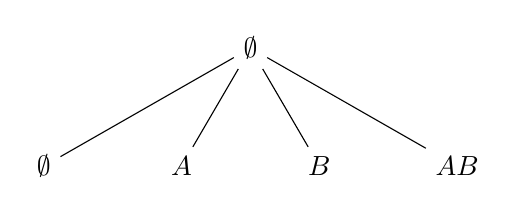
\begin{tikzpicture}[level distance=1.5cm,
    level 1/.style={sibling distance=1.75cm},
    level 2/.style={sibling distance=1.75cm}]
    \node {$\emptyset$}
        child {node {$\emptyset$}}
        child {node {$A$}}
        child {node {$B$}}
        child {node {$AB$}
        };
\end{tikzpicture}
\end{center} 
For each of the leaves in the above tree, possible combinations would be considered
for $t_3$.\\\\
With the exception of the $\emptyset$, each other node in the tree incurs a penalty
to the servers total broadcast count, $k$, equal to the number of pages broadcasted.
As a result, certain paths may run out of available broadcasts prematurely.  This 
provides justification for the following pruning rule.
\begin{prune}
If $k_{current} = 0$ for a given node prior to $t_{final}+1$, that node can be
pruned because it will be unable to satisfy any requests made from $t_{current}$ 
forward.  
\end{prune}
Although this pruning rule will eliminate redundancy, its effectiveness depends 
upon the total time and the number of possible pages needed to be served.\\\\
In addition to the variation of the broadcast counter $k$ of the server,
the decision to broadcast or not at every time may result in pages being delayed,
or an increase in the wait time as a function of the number pages not served
and the total time since the page was requested.  Since different subsets of 
pages can be served at a given time, it is possible that different decisions
made by the server might produce identical results.  As an example, at time 
$t_2$ in the above table of requests, the server might decide to serve $0$ pages
or to serve only page $A$.  In both cases, the set of unsatisfied requests is $\{B\}$.
As a result, the total wait that would carry over as a result of these decisions
is the same.
However, the decision to not broadcast does not deduct from the broadcast counter
of the server.  As a result, another pruning rule can be developed. 
\begin{prune}
If the total total number of unsatisfied requests at two nodes that made
different broadcasts decisions in the enumeration tree is the same, the
node that has the lower broadcast counter, $k$, can pruned.  If both nodes
have the same broadcast counter, the pruning can be done arbitrarily.
\end{prune}
This pruning rule guarantees that at every level, only the best choice
for a given accumulated wait is taken.  As a result, only one choice
will exist for each possible total delay.  Additionally, if the pruning
is done arbitrarily as a result of the broadcast counter being equal
amongst two nodes, the subsequence decision made from those nodes will
all add the same values to identical current delays.\\\\
Although the second pruning rule significantly reduces the number of nodes
at each level, this process requires considering all possible subsets of
size $k$ at every level.  Given a set of pages $\mathcal{P}$ with cardinality
$p$, this results in $2^{k}\binom nk$ possible subsets.  Attempting to 
search through all these subsets to find the correct subset of each size to consider
broadcasting at each level would lead to an exponentially running algorithm
dependent on $k$.\\\\
To solve this problem a separate dynamic programming problem can be sovled
to determine which subsets of each size should be considered.  In this 
subproblem, the possible subsets of size $l\ through\  k$ can be enumerated.
Broadcasting different subsets of each cardinality can lead to a different
number of unsatisfied requests.  This enables the following pruning condition
for this subproblem.
\begin{prune}
If two nodes have the same number of requests unsatisfied after serving
the same number of pages, prune a node arbitrarily since the remaining
unsatified pages will only go down by the same remaining possibilities
in either case.
\end{prune}
Applying this pruning rule to this problem results in only one leaf for
each possible wait time for each cardinality.  For each cardinality
considered, only the subset that minimizes the total number of unsatisfied 
requests needs to be considered.\\\\
Combining the two pruning rules for the overall problem and the rule
for the subproblem gives the following algorithm.\\\\
\begin{algorithm}[H]
\SetKw{Func}{Function: }
\SetKw{Inp}{Input: }
\SetKw{Init}{Initialization: }
\SetKw{EndInit}{End Initialization}
\SetKw{Glob}{Globals:}
\SetKw{Ret}{Return:}
\Func{MultiBroadCast}\\
\Inp{$T_{requests}$, $k$}\\
\Glob{$A[\ ][\ ][\ ]$}\\
\For{$i=2$ to $t_f$}
    {\For{$j=0$ to $k$}
        {\For{$l=0$ to $k$}
           { 
         \If{$A[i][j][l]$ is defined}
            {
                $subset_delay = FindSubset(T_{requests}[i],l)$
                $A[i+1][j+1][l+1] = \min(A[i][j+1][l+1], subset_i + A[i][j][l])$
            }
        }
    }
    }
\Ret{$\min(A[t_f][*][*])$}\\
\Func{FindSubset}\\
\Inp{$Array_{page}$, $l$}\\
\Glob{$A[\ ][\ ]$}\\
\For{$i=0$ to $n$}
    {\For{$j=0$ to $l$}
        {
            \If{$A[i][j]$ is defined}
                {
                    $delay = A[i][j] - Array_{page}[i]$
                    $A[i+1][delay] = j$
                }
        }
    }
\Ret{$\min(Array_{page}[n][*]$}
\end{algorithm} 
Although the \textit{FindSubset} function searches for the optimal subset
at a given time, it does not need to return the actual subset.  By 
returning only the value to the main function, the delay can be properly
accumulated.\\\\
To recover the broadcast times from the main program, the minimum total
wait time is found in the lowest row of the table.  This value can then 
be traced backward to see when the accumulated delay dropped to zero
and for which pages.  These points indicate the times at which the
server performed a broadcast and the pages served will have the requests
for those pages cleared.  This process can be repeated till time $t_1$.\\\\
The runtime for this algorithm is \BigO{nk^{3}t} due to the necessary
subset search by dynamic programming.
\end{document}
